\subsection{Make your data available}
    
As mentioned in the introduction to this chapter, original datasets may be available online. However, this doesn't necessarily
mean that they are readily \emph{accessible} to average users, for the following reasons:

\begin{itemize}
    \item \textbf{Location}. Datasets are usually available in open data portals that have been organized and structured not for ease of use, but according to some
          organisational convenience. 
          Despite more companies attempting to offer functional and efficient user interfaces, often a complicated search and selection process is necessary for a user to find what they need.
          Sometimes the data may not all be available in the one location, but may require searching through multiple portals.

    \item \textbf{Extraction}. Datasets are often available through an API (Application Programming Interface). Using an API requires specialist knowledge.
          Hopefully there will be a document describing the fields and values presented, and indicating how to actually use the API, but this is not guaranteed.

    \item \textbf{Readability}. Datasets are usually represented in a format designed to be processed by software. This is fairly unintelligible to a human user. At best,
          the data will be represented in a table and even then, it will often be quite difficult to extract the required information.
\end{itemize}

\subsubsection*{Suggested strategies} 

\begin{itemize}
    \item Provide the information required by the user in an uncomplicated manner, in a format that is easy to read and interpret,
          and we describe it in a way that is easy to understand and quick to digest.\\
\end{itemize}
 
\subsubsection*{In the context of Aire Guru \ldots} 

Our website uses the air quality data provided by the city of Málaga in its open data portal.(https://datosabiertos.malaga.eu/)\\

\begin{figure}[ht]
    \centering
    \subfigure[Main page]
        {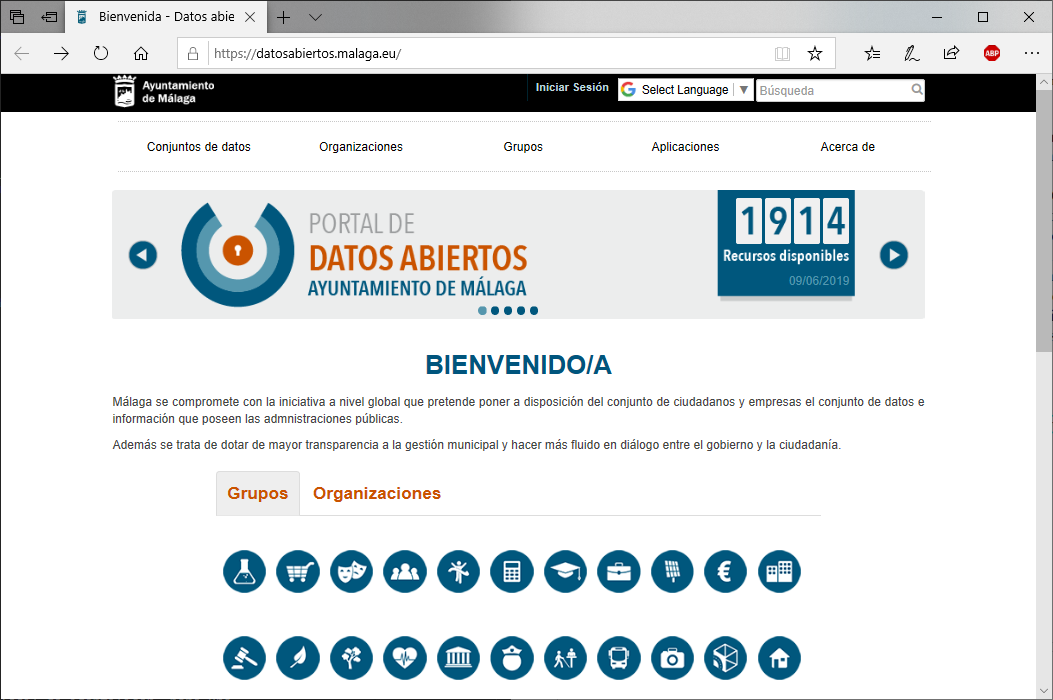
\includegraphics[width=5.5cm]{Figure_4_1_1_a_openDataPortal_mainPage}}
    \hfill
    \subfigure [Category environment]
        {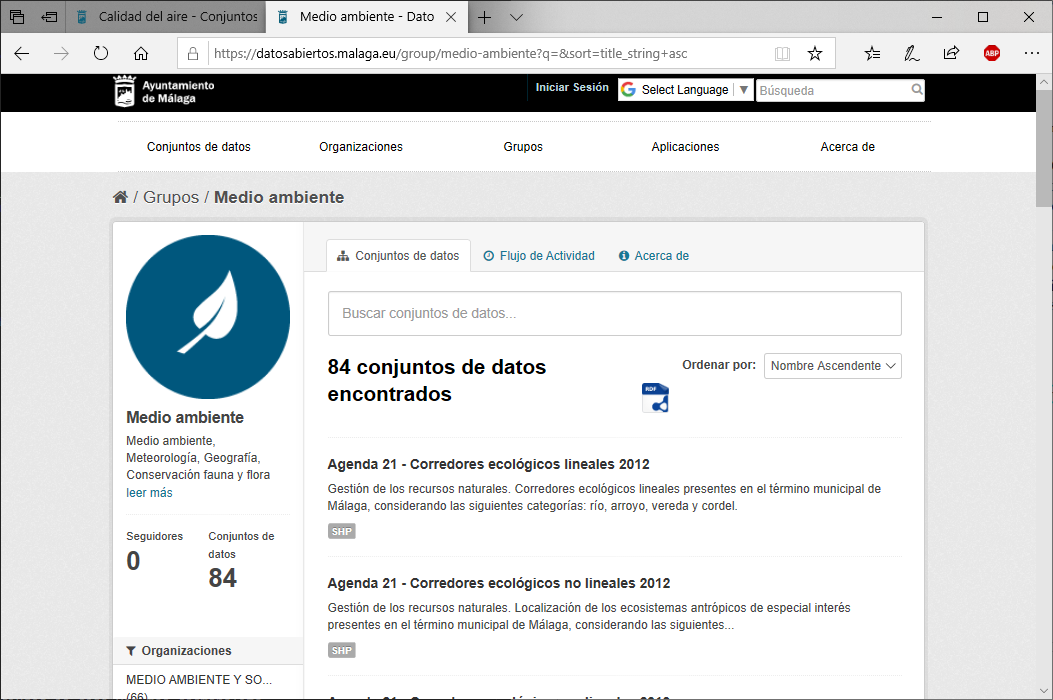
\includegraphics[width=5.5cm]{Figure_4_1_1_b_openDataPortalEnviromentCategory}}
    \vfill
    \subfigure[GeoJSON Document]
        {\centering 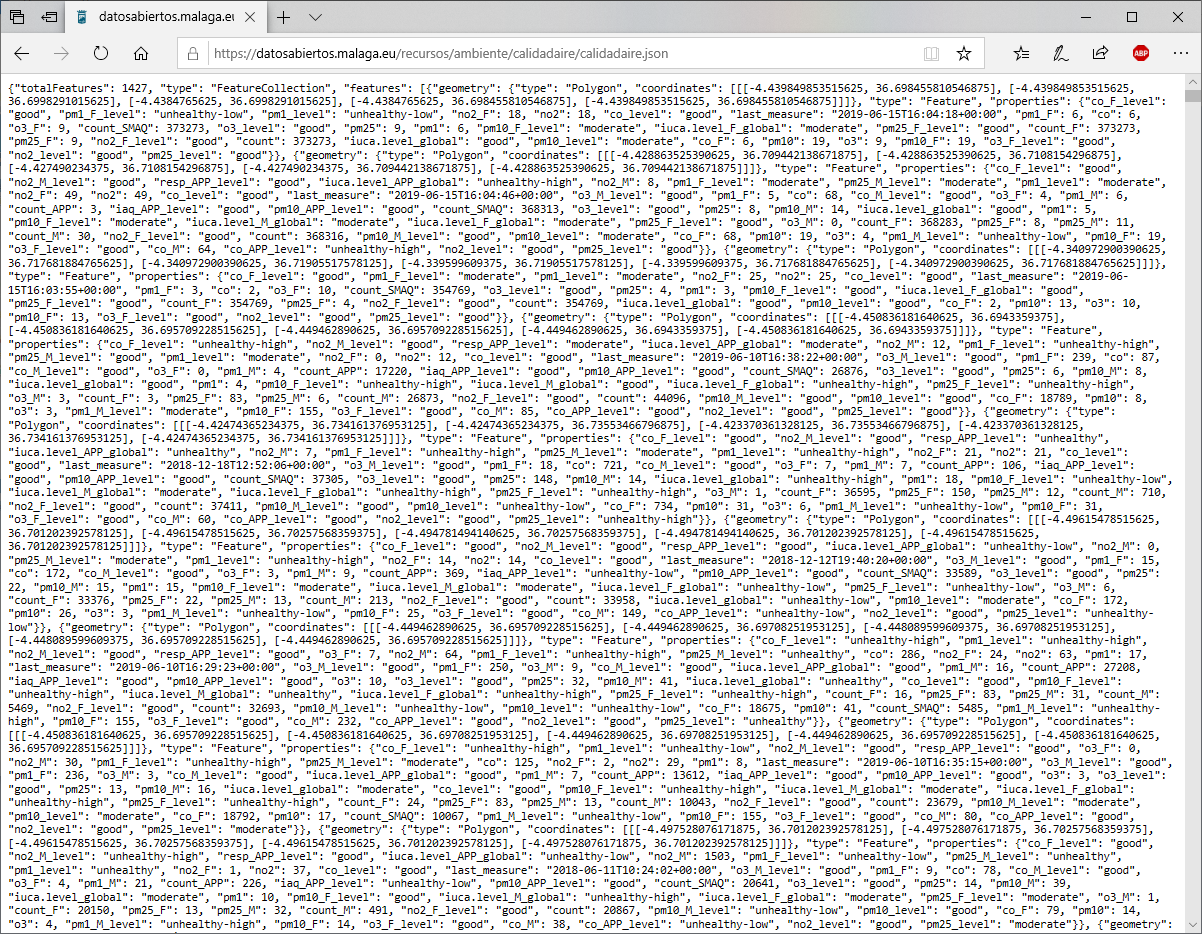
\includegraphics[width=4.75cm]{Figure_4_1_1_c_geoJsonDocument}}
    \caption{Open Data Portal Málaga}
\end{figure}


\begin{center}
    \bf{ (a) Main page     (b)Category environment\\
    (c)GeoJSONDocument
        
    Figure 4.1.1. Malaga's open data portal}
\end{center}

This data portal offers a variety of categories (represented by different icons) indicating classifications of the dataset.
Once a category is selected, the user is presented with a search bar that allows them to search for specific data using keywords.
In this case, if we click on the link, data is displayed in a new tab. The use of software
for translating the data is not strictly necessary, but we can see that the format (JSON) is not easily readable in human terms.
Aire Guru offers all the necessary information on a web platform which has been designed to facilitate human understanding. \\